\section{取整函数}
\begin{definition}[取整函数]
设\(x\in\mathbb{R},
n\in\mathbb{Z}\),
定义:\begin{enumerate}
	\item 如果\(n\)是不大于\(x\)的最大整数,
	即\(x\in[n,n+1)\),
	那么记\(\floor{x}=n\)\footnote{有的书把不大于\(x\)的最大整数
	称为“\(x\)的\DefineConcept{整数部分}”,记作\([x]\);
	把\(x\)与其整数部分之差\(x - [x]\)
	称为“\(x\)的\DefineConcept{小数部分}”,记作\(\{x\}\).}.
	我们把函数\(y=\floor{x}\)称为\DefineConcept{向下取整函数},
	即\begin{equation}
		\floor{x}
		\defeq
		\max\Set{ n\in\mathbb{Z} \given n \leq x }.
	\end{equation}

	\item 如果\(n\)是不小于\(x\)的最小整数,
	即\(x\in(n-1,n]\),
	那么记\(\ceil{x}=n\).
	我们把函数\(y=\ceil{x}\)称为\DefineConcept{向上取整函数},
	即\begin{equation}
		\ceil{x}
		\defeq
		\min\Set{ n\in\mathbb{Z} \given n \geq x }.
	\end{equation}
\end{enumerate}
\end{definition}

\begin{figure}[htb]
	\tikzstyle{sx}=[draw=orange,fill=orange]
	\tikzstyle{kx}=[draw=orange,fill=white]
	\def\subwidth{.45\linewidth}
	\def\subscale{.9}
	\begin{subfigure}[b]{\subwidth}%
		\centering
		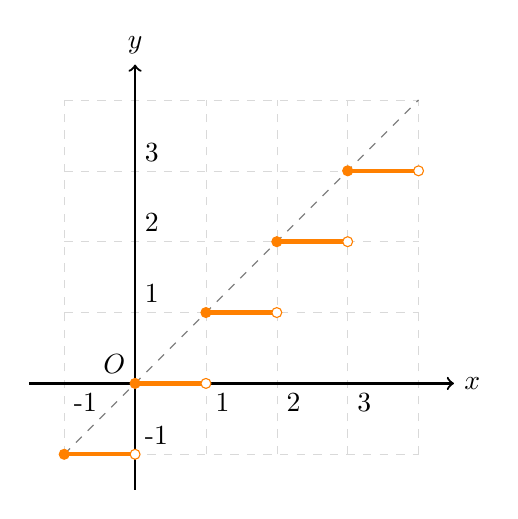
\begin{tikzpicture}[scale=\subscale]
			\draw[help lines, color=gray!30, dashed] (-1,-1) grid (4,4);
			\draw[dashed, color=gray] (-1,-1) -- (4,4);
			\draw[->, thick] (-1.5,0) -- (4.5,0) node[right]{\(x\)};
			\draw[->, thick] (0,-1.5) -- (0,4.5) node[above]{\(y\)};
			\foreach \i in {-1,...,3} {
				\draw[ultra thick,orange] (\i,\i)--(\i+1,\i);
				\fill[sx] (\i,\i)circle(2pt);
				\fill[kx] (\i+1,\i)circle(2pt);
				\ifnum\i=0\relax\else
					\draw(\i,0)node[below right]{\i};
					\draw(0,\i)node[above right]{\i};
				\fi
			}
			\draw (0,0)node[above left]{\(O\)};
		\end{tikzpicture}
		\subcaption{向下取整函数\(\floor{x}\)}
	\end{subfigure}
	\begin{subfigure}[b]{\subwidth}%
		\centering
		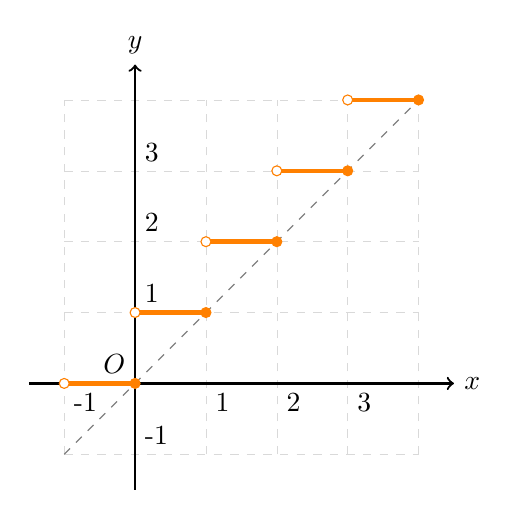
\begin{tikzpicture}[scale=\subscale]
			\draw[help lines, color=gray!30, dashed] (-1,-1) grid (4,4);
			\draw[dashed, color=gray] (-1,-1) -- (4,4);
			\draw[->, thick] (-1.5,0) -- (4.5,0) node[right]{\(x\)};
			\draw[->, thick] (0,-1.5) -- (0,4.5) node[above]{\(y\)};
			\foreach \i in {-1,...,3} {
				\draw[ultra thick,orange] (\i,\i+1)--(\i+1,\i+1);
				\fill[kx] (\i,\i+1)circle(2pt);
				\fill[sx] (\i+1,\i+1)circle(2pt);
				\ifnum\i=0\relax\else
					\draw(\i,0)node[below right]{\i};
					\draw(0,\i)node[above right]{\i};
				\fi
			}
			\draw (0,0)node[above left]{\(O\)};
		\end{tikzpicture}
		\subcaption{向上取整函数\(\ceil{x}\)}
	\end{subfigure}
	\caption{取整函数的图形}
	\label{figure:取整函数.取整函数的图形}
\end{figure}

\begin{figure}
	\tikzstyle{sx}=[draw=orange,fill=orange]
	\tikzstyle{kx}=[draw=orange,fill=white]
	\def\subwidth{.45\linewidth}
	\def\subscale{.9}
	%@Mathematica: Plot[x - Floor[x], {x, -1, 4}]
	%@Mathematica: Table[{x, x - Floor[x]}, {x, -1, 4, .2}] // TableForm
	\begin{subfigure}[b]{\subwidth}%
		\centering
		\begin{tikzpicture}[scale=\subscale]
			\begin{axis}[
				xmin=-1,xmax=4,
				ymin=-1,ymax=1,
				restrict y to domain=-1:1,
				axis lines=middle,
				axis equal=true,
				xlabel=$x$,
				ylabel=$y$,
				enlarge x limits=0.1,
				enlarge y limits=0.1,
				x label style={at={(ticklabel* cs:1.00)}, inner sep=5pt, anchor=south},
				y label style={at={(ticklabel* cs:1.00)}, inner sep=2pt, anchor=west},
				ytick={-1,1},
			]
				\foreach \i in {-1,...,3} {
					\addplot[color=orange,samples=2,domain={\i}:{\i+1}]{x-\i};
				}
				\fill[kx](-1,1)circle(2pt);
				\fill[kx](0,1)circle(2pt);
				\fill[kx](1,1)circle(2pt);
				\fill[kx](2,1)circle(2pt);
				\fill[kx](3,1)circle(2pt);
				\fill[kx](4,1)circle(2pt);
				\fill[sx](-1,0)circle(2pt);
				\fill[sx](0,0)circle(2pt);
				\fill[sx](1,0)circle(2pt);
				\fill[sx](2,0)circle(2pt);
				\fill[sx](3,0)circle(2pt);
				\fill[sx](4,0)circle(2pt);
			\end{axis}
		\end{tikzpicture}
		\subcaption{函数\(f(x)=x-\floor{x}\)}
	\end{subfigure}
	%@Mathematica: Plot[Ceiling[x] - x, {x, -1, 4}]
	%@Mathematica: Table[{x, Ceiling[x] - x}, {x, -1, 4, .2}] // TableForm
	\begin{subfigure}[b]{\subwidth}%
		\centering
		\begin{tikzpicture}[scale=\subscale]
			\begin{axis}[
				xmin=-1,xmax=4,
				ymin=-1,ymax=1,
				axis lines=middle,
				axis equal=true,
				xlabel=$x$,
				ylabel=$y$,
				enlarge x limits=0.1,
				enlarge y limits=0.1,
				x label style={at={(ticklabel* cs:1.00)}, inner sep=5pt, anchor=south},
				y label style={at={(ticklabel* cs:1.00)}, inner sep=2pt, anchor=west},
				ytick={-1,1},
			]
				\foreach \i in {-1,...,3} {
					\addplot[color=orange,samples=2,domain={\i}:{\i+1}]{\i+1-x};
				}
				\fill[kx](-1,1)circle(2pt);
				\fill[kx](0,1)circle(2pt);
				\fill[kx](1,1)circle(2pt);
				\fill[kx](2,1)circle(2pt);
				\fill[kx](3,1)circle(2pt);
				\fill[kx](4,1)circle(2pt);
				\fill[sx](-1,0)circle(2pt);
				\fill[sx](0,0)circle(2pt);
				\fill[sx](1,0)circle(2pt);
				\fill[sx](2,0)circle(2pt);
				\fill[sx](3,0)circle(2pt);
				\fill[sx](4,0)circle(2pt);
			\end{axis}
		\end{tikzpicture}
		\subcaption{函数\(f(x)=\ceil{x}-x\)}
	\end{subfigure}
	\caption{}
\end{figure}

\begin{property}\label{theorem:取整函数.性质1}
%@see: 《算法导论(原书第3版)》 P31 (3.3)
%@see: 《具体数学 计算机科学基础(第2版)》 P57 (3.3)
一般地,对于\(x\in\mathbb{R}\),总有\begin{equation}
	x - 1 < \floor{x} \leq x \leq \ceil{x} < x + 1.
\end{equation}
当且仅当\(x\)是整数时,
成立\(x = \ceil{x} = \floor{x}\).
%TODO proof
\end{property}

\begin{property}
%@see: 《具体数学 计算机科学基础(第2版)》 P57 (3.4)
设\(x\)是实数,则\begin{gather}
	\floor{-x} = -\ceil{x},
	\label{equation:取整函数.取整函数的对称性1} \\
	\ceil{-x} = -\floor{x}.
	\label{equation:取整函数.取整函数的对称性2}
\end{gather}
%TODO proof
\end{property}
\begin{remark}
从\cref{figure:取整函数.取整函数的图形} 可以看出:
函数\(\ceil{x}\)与\(\floor{x}\)的图形关于坐标原点\(O\)中心对称.
\end{remark}

\begin{property}
%@see: 《具体数学 计算机科学基础(第2版)》 P57 (3.5)
设\(x\)是实数,\(n\)是整数,则\begin{gather}
	\floor{x} = n
	\iff
	n \leq x < n+1
	\iff
	x-1 < n \leq x,
	\label{equation:取整函数.序关系1} \\
	\ceil{x} = n
	\iff
	n-1 < x \leq n
	\iff
	x \leq n < x+1.
	\label{equation:取整函数.序关系2}
\end{gather}
%TODO proof
\end{property}

\begin{example}
设\(x,y\)都是实数.
举例说明:\(\ceil{x} + \ceil{y} \neq \ceil{x+y},
\floor{x} + \floor{y} \neq \floor{x+y}\).
\begin{solution}
%@credit: {6d916ea6-1441-4c5b-9e97-4f834b319710} 说:都取0.5
取\(x = y = \frac12\).
那么\(\ceil{x} = \ceil{y} = \ceil{x+y} = 1\),
但是\(\ceil{x} + \ceil{y} = 2 \neq \ceil{x+y}\).

与此同时,\(\floor{x} = \floor{y} = 0,
\floor{x+y} = 1\),
因此\(\floor{x} + \floor{y} \neq \floor{x+y}\).
\end{solution}
\end{example}
\begin{example}
设\(x,y\)都是实数.
举例说明:\(\ceil{xy} \neq x\ceil{y},
\floor{xy} \neq x\floor{y}\).
\begin{solution}
取\(x=2,y=\frac12\).
那么\(\ceil{xy} = 1 \neq x\ceil{y} = 2,
\floor{xy} = 1 \neq x\ceil{y} = 0\).
\end{solution}
\end{example}

\begin{proposition}
%@see: 《具体数学 计算机科学基础(第2版)》 P58 (3.6)
设\(n\)是整数,\(x\)是实数,则\begin{gather*}
	\ceil{n+x} = n + \ceil{x},
	\label{equation:取整函数.取整函数的周期性1} \\
	\floor{n+x} = n + \floor{x}.
	\label{equation:取整函数.取整函数的周期性2}
\end{gather*}
%TODO proof
% \begin{proof}
% % 因为\begin{align*}
% % 	\floor{x} = n
% % 	\iff
% % 	n \leq x < n+1
% % 	\iff
% % 	\floor{x}+n \leq x+n < \floor{x}+n+1
% % 	\iff
% % 	\floor{x+n} = \floor{x}+n.
% % \end{align*}
% 由定义可知\begin{align*}
% 	\floor{n+x}
% 	&= \max\Set{ m\in\mathbb{Z} \given m \leq n+x } \\
% 	&= \max\Set{ m\in\mathbb{Z} \given m-n \leq x } \\
% 	&= \max\Set{ m\in\mathbb{Z} \given k=m-n, k \leq x } \\
% 	&= \max\Set{ m\in\mathbb{Z} \given m=n+k, k \leq x } \\
% 	%TODO 这里其实还没有说清楚
% 	&= n + \max\Set{ k\in\mathbb{Z} \given k \leq x } \\
% 	&= n + \floor{x}.
% \end{align*}
% 同理可知\(\ceil{n+x} = n + \ceil{x}\).
% \end{proof}
\end{proposition}

\begin{property}
%@see: 《具体数学 计算机科学基础(第2版)》 P58 (3.7)
设\(x\)是实数,\(n\)是整数,则\begin{gather}
	x < n \iff \floor{x} < n,
	\label{equation:取整函数.序关系3} \\
	n < x \iff n < \ceil{x},
	\label{equation:取整函数.序关系4} \\
	x \leq n \iff \ceil{x} \leq n,
	\label{equation:取整函数.序关系5} \\
	n \leq x \iff n \leq \floor{x}.
	\label{equation:取整函数.序关系6}
\end{gather}
%TODO proof
\begin{proof}
% 证明\(x < n \iff \floor{x} < n\):
证明\cref{equation:取整函数.序关系3}:
当\(x < n\)时,
%\cref{theorem:取整函数.性质1}
由\(\floor{x} \leq x\)
可得\(\floor{x} < n\).
当\(\floor{x} < n\)时,
%\cref{equation:取整函数.序关系1}
由\(x < \floor{x} + 1\)
%@credit: {57e837df-6d92-457b-a5f0-e915ab36f532},{5f4d2f8a-fc8b-4798-85d6-98670f6761e7} 说:
% \(\floor{x}\)作为一个整数,小于另一个整数\(n\),那么必有\(\floor{x} + 1 \leq n\)
和\(\floor{x} + 1 \leq n\)
可得\(x < n\).

% 证明\(n < x \iff n < \ceil{x}\):
证明\cref{equation:取整函数.序关系4}:
当\(n < x\)时,
%\cref{theorem:取整函数.性质1}
由\(x \leq \ceil{x}\)
可得\(n < \ceil{x}\).
当\(n < \ceil{x}\)时,
% \(\ceil{x}\)作为一个整数,大于另一个整数\(n\),那么必有\(n + 1 \leq \ceil{x}\)
由\(n \leq \ceil{x} - 1\)
%\cref{equation:取整函数.序关系2}
和\(\ceil{x} - 1 < x\)
可得\(n < x\).

同理可证\cref{equation:取整函数.序关系5,equation:取整函数.序关系6}.
\end{proof}
\end{property}

\begin{proposition}
%@see: 《具体数学 计算机科学基础(第2版)》 P59
设\(x\)是实数,则\begin{gather*}
	\ceil{\floor{x}} = \floor{x}, \\
	\floor{\floor{x}} = \floor{x}, \\
	\ceil{\ceil{x}} = \ceil{x}, \\
	\floor{\ceil{x}} = \ceil{x}.
\end{gather*}
\begin{proof}
因为\(\floor{x},\ceil{x}\)都是整数,
所以由\cref{theorem:取整函数.性质1} 可知,
对它们两个而言,不论向上取整还是向下取整,都不会发生变化.
\end{proof}
\end{proposition}

\begin{example}\label{example:取整函数.根式函数与取整函数的复合}
%@see: 《具体数学 计算机科学基础(第2版)》 P59 (3.9)
设\(x\)是非负实数.
证明:\begin{gather}
	\floor{\sqrt{\floor{x}}} = \floor{\sqrt{x}}, \\
	\ceil{\sqrt{\ceil{x}}} = \ceil{\sqrt{x}}.
\end{gather}
\begin{proof}
设\(m = \floor{\sqrt{\floor{x}}}\).
由\cref{equation:取整函数.序关系1}
可知\(m \leq \sqrt{\floor{x}} < m+1\).
因为\(m \geq 0\),
%@credit: {3b700f59-6290-449f-8174-9204a938f47c} 帮忙发现了一个 typo
所以\begin{equation*}
	m^2 \leq \floor{x} < (m+1)^2.
\end{equation*}
由\cref{equation:取整函数.序关系6}
可知\(m^2 \leq x\);
由\cref{equation:取整函数.序关系3}
可知\(x < (m+1)^2\);
因此\(m^2 \leq x < (m+1)^2\),
从而有\(m \leq \sqrt{x} < m+1\),
即\(m = \floor{\sqrt{x}}\).
总之,我们有\(\floor{\sqrt{\floor{x}}} = \floor{\sqrt{x}}\).
同理可证\(\ceil{\sqrt{\ceil{x}}} = \ceil{\sqrt{x}}\).
\end{proof}
\end{example}
接下来对\cref{example:取整函数.根式函数与取整函数的复合} 的结论进行推广.
\begin{example}\label{example:取整函数.单调增加函数与取整函数的复合}
%@see: 《具体数学 计算机科学基础(第2版)》 P60 (3.10)
对于任意一个在实数区间内连续的单调增加函数\(f\),
只要它满足\begin{equation*}
	(\forall x)[f(x) \in \mathbb{Z} \implies x \in \mathbb{Z}],
\end{equation*}
那么当\(f(x),f(\floor{x}),f(\ceil{x})\)三者均有定义时,
成立\(\floor{f(x)} = \floor{f(\floor{x})}\)
和\(\ceil{f(x)} = \ceil{f(\ceil{x})}\).
\begin{proof}
当\(x = \ceil{x}\)时,显然成立\(\ceil{f(x)} = \ceil{f(\ceil{x})}\).

当\(x \neq \ceil{x}\)时,
必然成立\(x < \ceil{x}\).
因为函数\(f\)是单调增加的,
所以\(f(x) < f(\ceil{x})\).
因为函数\(x \mapsto \ceil{x}\)单调不减,
所以\(\ceil{f(x)} \leq \ceil{f(\ceil{x})}\).

接下来用反证法,
假设\(\ceil{f(x)} < \ceil{f(\ceil{x})}\).
\begin{figure}
	\tikzstyle{sx}=[draw=orange,fill=orange]
	\tikzstyle{kx}=[draw=orange,fill=white]
	\centering
	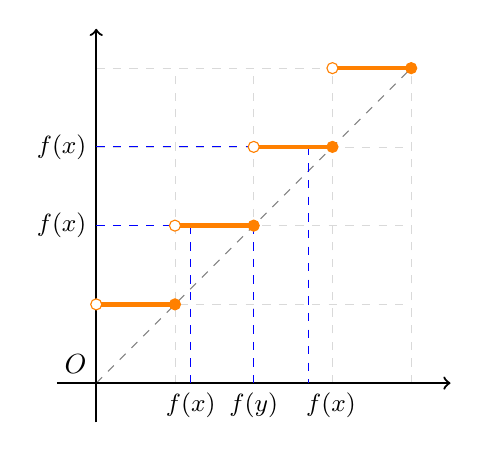
\begin{tikzpicture}
		\draw[help lines, color=gray!30, dashed] (0,0) grid (4,4);
		\draw[dashed, color=gray] (0,0) -- (4,4);
		\draw[->, thick] (-.5,0) -- (4.5,0);
		\draw[->, thick] (0,-.5) -- (0,4.5);

		\draw[blue,dashed] (0,2)--(1,2) (0,3)--(2,3);
		\draw[blue,dashed] (1.2,2)--(1.2,0)node[black,below]{\small$f(x)$}
					(2,2)--(2,0)node[black,below]{\small$f(y)$}
					(2.7,3)--(2.7,0)++(8pt,0)node[black,below]{\small$f(\ceil{x})$};
		\draw (0,2)node[left]{\small$\ceil{f(x)}$}
			(0,3)node[left]{\small$\ceil{f(\ceil{x})}$};

		\foreach \i in {0,...,3} {
			\draw[ultra thick,orange] (\i,\i+1)--(\i+1,\i+1);
			\fill[kx] (\i,\i+1)circle(2pt);
			\fill[sx] (\i+1,\i+1)circle(2pt);
		}
		\draw (0,0)node[above left]{\(O\)};
	\end{tikzpicture}
	\caption{}
	\label{figure-example:取整函数.单调增加函数与取整函数的复合}
\end{figure}
由于\(f\)是连续的单调增加函数,
如\cref{figure-example:取整函数.单调增加函数与取整函数的复合} 所示,
那么必定存在实数\(y\)
满足\(x \leq y < \ceil{x}\),
并使得\(f(y) = \ceil{f(x)}\).
因为\(\ceil{f(x)}\)是一个整数,
那么由前提条件\((\forall x)[f(x) \in \mathbb{Z} \implies x \in \mathbb{Z}]\)
可知\(y\)只能是整数.
然而不可能有一个整数严格位于\(\floor{x}\)与\(\ceil{x}\)之间.
这个矛盾说明\(\ceil{f(x)} = \ceil{f(\ceil{x})}\)必定成立.

同理可证\(\floor{f(x)} = \floor{f(\floor{x})}\).
\end{proof}
\end{example}
\begin{example}
%@see: 《具体数学 计算机科学基础(第2版)》 P60 (3.11)
设\(x\)是实数,\(m,n\)都是整数,且\(n>0\),
则\begin{gather}
	\floor*{\frac{x+m}{n}} = \floor*{\frac{\floor{x}+m}{n}}, \\
	\ceil*{\frac{x+m}{n}} = \ceil*{\frac{\ceil{x}+m}{n}}.
\end{gather}
\begin{proof}
令\(f(x) = \frac{x+m}{n}\),
由\cref{example:取整函数.单调增加函数与取整函数的复合} 可得.
\end{proof}
\end{example}
\begin{example}
%@see: 《具体数学 计算机科学基础(第2版)》 P60
设\(x\)是非负实数.
举例说明:\(\ceil{\sqrt{\floor{x}}} \neq \ceil{\sqrt{x}}\).
\begin{solution}
取\(x = \frac{1+\sqrt5}2\).
%@Mathematica: Ceiling[Sqrt[Floor[x]]] /. x -> GoldenRatio
%@Mathematica: Ceiling[Sqrt[x]] /. x -> GoldenRatio
那么\(\ceil{\sqrt{\floor{x}}} = 1 \neq \ceil{\sqrt{x}} = 2\).
\end{solution}
\end{example}
\begin{example}
%@see: 《具体数学 计算机科学基础(第2版)》 P61
设\(x\)是非负实数.
证明:\(\ceil{\sqrt{\floor{x}}} = \ceil{\sqrt{x}}\)
当且仅当\(x\)是整数,或\(\sqrt{\floor{x}}\)是整数.
%TODO proof
\end{example}
\begin{example}
%@see: 《具体数学 计算机科学基础(第2版)》 P61
设\(a,b\)都是整数.
记\(\card_X Y \defeq \card\Set{ x \in X \given x \in Y }\).
证明:\begin{equation*}
	\card_\mathbb{Z} [a,b)
	= \card_\mathbb{Z} (a,b]
	= b-a.
\end{equation*}
%TODO proof
\end{example}
\begin{example}
%@see: 《具体数学 计算机科学基础(第2版)》 P61
设\(a,b\)都是实数.
证明:\begin{gather*}
	\card_\mathbb{Z} [a,b)
	= \ceil{b} - \ceil{a}, \\
	\card_\mathbb{Z} (a,b]
	= \floor{b} - \floor{a}, \\
	\card_\mathbb{Z} [a,b]
	= \floor{b} - \ceil{a} + 1, \\
	\card_\mathbb{Z} (a,b)
	= \ceil{b} - \floor{a} - 1.
\end{gather*}
%TODO proof
\begin{proof}
由\cref{equation:取整函数.序关系6} 可知,
对于任意整数\(n\)和任意实数\(\alpha,\beta\),
有\begin{gather*}
	\alpha \leq n < \beta
	\iff
	\ceil{\alpha} \leq n < \ceil{\beta}, \\
	\alpha < n \leq \beta
	\iff
	\ceil{\alpha} < n \leq \ceil{\beta}.
\end{gather*}
\let\qed\relax
\end{proof}
\end{example}

\begin{property}
%@see: 《算法导论(原书第3版)》 P31
对于\(n\in\mathbb{Z}\),总有\begin{equation}
	\ceil{n/2} + \floor{n/2} = n.
\end{equation}
\begin{proof}
%@credit: {8b6edada-f2fd-4ae5-9020-eb533149a54c} 说可以分为n是偶数或n是奇数两种情况讨论
当\(n\)是偶数时,
存在整数\(k\)使得\(n=2k\),
那么\begin{equation*}
	\ceil{n/2} = \floor{n/2} = k,
\end{equation*}
于是\(\ceil{n/2} + \floor{n/2} = 2k = n\).

当\(n\)是奇数时,
存在整数\(k\)使得\(n=2k+1\),
即有\(n/2 = k + 1/2\),
那么\begin{equation*}
	\ceil{n/2} = k+1,
	\qquad
	\floor{n/2} = k,
\end{equation*}
于是\(\ceil{n/2} + \floor{n/2} = 2k+1 = n\).
\end{proof}
\end{property}

\begin{property}
%@see: 《算法导论(原书第3版)》 P31 (3.4)
%@see: 《算法导论(原书第3版)》 P31 (3.5)
%@see: 《算法导论(原书第3版)》 P31 (3.6)
%@see: 《算法导论(原书第3版)》 P31 (3.7)
对于任意实数\(x \geq 0\)和整数\(a,b>0\),总有\begin{gather}
	\ceil*{\frac{\ceil{x/a}}{b}} = \ceil*{\frac{x}{ab}}, \\
	\floor*{\frac{\floor{x/a}}{b}} = \floor*{\frac{x}{ab}}, \\
	\ceil*{\frac{a}{b}} \leq \frac{a+(b-1)}{b}, \\
	\floor*{\frac{a}{b}} \geq \frac{a-(b-1)}{b}.
\end{gather}
%TODO proof
\end{property}

\begin{example}
证明:对于任意整数\(n\),
总有\(\ceil*{\frac{n}2\vphantom{\frac12}} = \floor*{\frac{n+1}2}\).
%TODO proof
\end{example}
\begin{example}
证明:对于任意整数\(n,m\),
总有\(\ceil*{\frac{n}{m}\vphantom{\frac12}} = \floor*{\frac{n+m-1}{m}}\).
%TODO proof
\end{example}
